
%(BEGIN_QUESTION)
% Copyright 2010, Tony R. Kuphaldt, released under the Creative Commons Attribution License (v 1.0)
% This means you may do almost anything with this work of mine, so long as you give me proper credit

This liquid level switch is mounted to the side of a pressurized process vessel, with two block valves for isolation, plus a drain and a vent valve.  The switch actuates when the process liquid level rises high enough to make the float buoyant:

$$\includegraphics[width=15.5cm]{i04745x01.eps}$$

Your task is to figure out how to ``trip'' this high-level alarm switch to test its operation, ensuring it still functions as it should, without disconnecting or removing any part of it from the process vessel.  Assume that the actual liquid level inside the process vessel is below the trip point, and cannot be raised to help you do this test.  In other words, you must devise an ``in-place'' test for the switch that may be performed at any time. 

\underbar{file i04745}
%(END_QUESTION)





%(BEGIN_ANSWER)

Shut the upper block valve and slowly open the vent valve, allowing process vapor pressure to push more liquid into the float chamber and raise the float.

\vskip 10pt

Alternatively, one could shut both block valves, open the vent valve, and pour in liquid until the float raises high enough to trip the switch.

\vskip 10pt

{\it If the student gives an answer describing how to electrically simulate the alarm (e.g. opening or shorting wires), give half credit.  This would test the shutdown system, but not the level switch specifically.}

%(END_ANSWER)





%(BEGIN_NOTES)

{\bf This question is intended for exams only and not worksheets!}

%(END_NOTES)


